\subsection{Full Sample Metrics}
Table~\ref{tab:all-metrics} supplements Table~\ref{tab:main} with distances, coverage, and validity.
\begin{table}[t]\caption{Additional controlled test metrics, mean $\pm$ training-seed SD for NN and coverage. Validity reports the mean error defined in the text.}\label{tab:all-metrics}\centering\small\begin{tabular}{@{}llrrr@{}}\toprule
Data & Method / updates & Symmetric NN $\downarrow$ & Coverage $\uparrow$ & Validity error $\downarrow$ \\
\midrule
Volcano & R-MGM mixture / 2k & $0.119\,\pm\,0.021$ & $0.028\,\pm\,0.019$ & $3.0e-08$ \\
Volcano & RFM / 2k & $0.204\,\pm\,0.003$ & $0.005\,\pm\,0.006$ & $3.3e-08$ \\
Volcano & RFM / 10k & $0.189\,\pm\,0.003$ & $0.005\,\pm\,0.005$ & $3.5e-08$ \\
Earthquake & R-MGM mixture / 2k & $0.044\,\pm\,0.001$ & $0.156\,\pm\,0.006$ & $3.2e-08$ \\
Earthquake & RFM / 2k & $0.101\,\pm\,0.000$ & $0.054\,\pm\,0.003$ & $3.5e-08$ \\
Earthquake & RFM / 10k & $0.079\,\pm\,0.001$ & $0.092\,\pm\,0.009$ & $3.5e-08$ \\
Flood & R-MGM mixture / 2k & $0.052\,\pm\,0.001$ & $0.123\,\pm\,0.022$ & $3.0e-08$ \\
Flood & RFM / 2k & $0.097\,\pm\,0.001$ & $0.062\,\pm\,0.004$ & $3.4e-08$ \\
Flood & RFM / 10k & $0.087\,\pm\,0.001$ & $0.073\,\pm\,0.012$ & $3.4e-08$ \\
Fire & R-MGM mixture / 2k & $0.028\,\pm\,0.002$ & $0.144\,\pm\,0.015$ & $3.0e-08$ \\
Fire & RFM / 2k & $0.087\,\pm\,0.001$ & $0.022\,\pm\,0.000$ & $3.5e-08$ \\
Fire & RFM / 10k & $0.067\,\pm\,0.002$ & $0.035\,\pm\,0.001$ & $3.4e-08$ \\
General & R-MGM mixture / 2k & $0.096\,\pm\,0.019$ & $0.198\,\pm\,0.092$ & $0.0e+00$ \\
General & RFM / 2k & $0.166\,\pm\,0.001$ & $0.203\,\pm\,0.010$ & $0.0e+00$ \\
General & RFM / 10k & $0.132\,\pm\,0.001$ & $0.269\,\pm\,0.006$ & $0.0e+00$ \\
Glycine & R-MGM mixture / 2k & $0.172\,\pm\,0.033$ & $0.091\,\pm\,0.043$ & $0.0e+00$ \\
Glycine & RFM / 2k & $0.161\,\pm\,0.002$ & $0.118\,\pm\,0.004$ & $0.0e+00$ \\
Glycine & RFM / 10k & $0.114\,\pm\,0.003$ & $0.238\,\pm\,0.006$ & $0.0e+00$ \\
Proline & R-MGM mixture / 2k & $0.136\,\pm\,0.011$ & $0.064\,\pm\,0.029$ & $0.0e+00$ \\
Proline & RFM / 2k & $0.230\,\pm\,0.002$ & $0.104\,\pm\,0.012$ & $0.0e+00$ \\
Proline & RFM / 10k & $0.101\,\pm\,0.007$ & $0.213\,\pm\,0.014$ & $0.0e+00$ \\
Pre-Pro & R-MGM mixture / 2k & $0.061\,\pm\,0.016$ & $0.316\,\pm\,0.062$ & $0.0e+00$ \\
Pre-Pro & RFM / 2k & $0.157\,\pm\,0.002$ & $0.204\,\pm\,0.006$ & $0.0e+00$ \\
Pre-Pro & RFM / 10k & $0.134\,\pm\,0.004$ & $0.246\,\pm\,0.026$ & $0.0e+00$ \\
RNA (7D) & R-MGM mixture / 2k & $0.396\,\pm\,0.002$ & $0.314\,\pm\,0.010$ & $0.0e+00$ \\
RNA (7D) & RFM / 2k & $0.965\,\pm\,0.004$ & $0.000\,\pm\,0.000$ & $0.0e+00$ \\
RNA (7D) & RFM / 10k & $0.736\,\pm\,0.013$ & $0.041\,\pm\,0.015$ & $0.0e+00$ \\
\bottomrule\end{tabular}\end{table}
Spherical NN units are radians. Torus NN uses the Euclidean norm of wrapped angular differences in radians. The coverage threshold is fixed separately per dataset from training data. Validity means unit-norm error on a sphere and out-of-range fraction on a torus; these different quantities must not be averaged across domains.
\subsection{Matched MLP Objective Controls}
Figure~\ref{fig:objective-controls} visualizes the parameterization-matched models from training seed 0.
\begin{figure}[t]\centering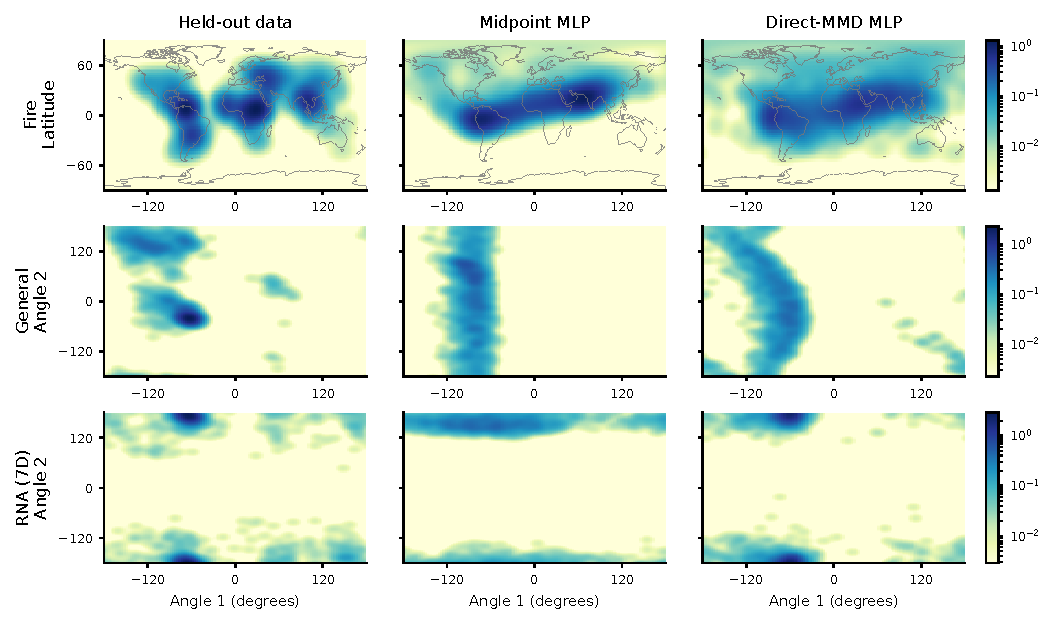
\includegraphics[width=\textwidth]{figures/objective_controls.pdf}
\caption{Matched constrained MLPs after 2,000 updates: the same fixed test targets and training seed 0, with midpoint and direct-MMD objectives. Each row uses one logarithmic KDE scale and the plotting convention of Figure~\ref{fig:controlled}. Only the first two RNA angles are displayed. These are sample densities, not model likelihoods.}\label{fig:objective-controls}\end{figure}
Table~\ref{tab:mlp-metrics} supplements the matched-architecture objective comparison with non-MMD metrics. The MMD control directly optimizes the evaluation kernel, so its MMD advantage alone would not establish superiority on all distributional criteria.
\begin{table}[t]\caption{Matched MLP controls at 2,000 generator updates. Mean and sample SD across three training seeds, after averaging three draws per seed. Smaller symmetric NN and larger coverage are better.}\label{tab:mlp-metrics}\centering\small\begin{tabular}{@{}llrr@{}}\toprule
Data & Objective & Symmetric NN & Coverage \\
\midrule
Fire & Midpoint & $0.115\,\pm\,0.011$ & $0.024\,\pm\,0.017$ \\
Fire & Direct MMD & $0.080\,\pm\,0.002$ & $0.030\,\pm\,0.004$ \\
General & Midpoint & $0.168\,\pm\,0.022$ & $0.196\,\pm\,0.026$ \\
General & Direct MMD & $0.158\,\pm\,0.004$ & $0.257\,\pm\,0.011$ \\
RNA (7D) & Midpoint & $0.913\,\pm\,0.225$ & $0.000\,\pm\,0.000$ \\
RNA (7D) & Direct MMD & $0.508\,\pm\,0.016$ & $0.111\,\pm\,0.039$ \\
\bottomrule\end{tabular}\end{table}
\subsection{Numerical Geometry Audits}
Table~\ref{tab:geometry-audit} reports the interpolation residuals.
\begin{table}[t]\caption{Maximum numerical residuals over 64 float64 endpoint pairs per geometry. Position and derivative-comparison norms are ambient; velocity reversal uses the manifold metric.}\label{tab:geometry-audit}\centering\small\begin{tabular}{@{}lrrr@{}}\toprule
Geometry & Position reversal & Velocity reversal & Velocity vs. finite difference \\
\midrule
sphere & $2.38e-14$ & $3.48e-15$ & $2.88e-10$ \\
torus & $1.28e-15$ & $0.00e+00$ & $5.36e-10$ \\
spd & $1.63e-15$ & $5.96e-16$ & $6.58e-10$ \\
hyperbolic & $7.09e-08$ & $8.02e-08$ & $8.37e-08$ \\
\bottomrule\end{tabular}\end{table}
The hyperbolic target itself is approximate. The audited endpoint distribution is not an exhaustive numerical guarantee.
\subsection{Empirical Training-Resampling Reference}
Table~\ref{tab:resampling} calibrates the sample estimator using direct resampling from the empirical training distribution. It is a memorization reference, not a learned generator or a universal lower bound on MMD.
\begin{table}[t]\caption{Empirical training resampling against the fixed test targets. Mean and Monte Carlo SD over three draws; there are zero training seeds in these reference rows.}\label{tab:resampling}\centering\small\begin{tabular}{@{}lrrr@{}}\toprule
Data & MMD$^2\times10^3$ & Symmetric NN & Coverage \\
\midrule
Volcano & $13.390\pm6.585$ & $0.062\pm0.004$ & $0.447\pm0.078$ \\
Earthquake & $1.632\pm0.658$ & $0.024\pm0.001$ & $0.381\pm0.030$ \\
Fire & $0.796\pm0.288$ & $0.012\pm0.001$ & $0.441\pm0.031$ \\
Flood & $1.833\pm1.152$ & $0.034\pm0.002$ & $0.324\pm0.016$ \\
General & $0.992\pm0.732$ & $0.037\pm0.001$ & $0.525\pm0.011$ \\
Glycine & $1.144\pm0.464$ & $0.054\pm0.000$ & $0.476\pm0.009$ \\
Proline & $0.499\pm0.242$ & $0.025\pm0.000$ & $0.421\pm0.007$ \\
Pre-Pro & $1.321\pm0.476$ & $0.040\pm0.002$ & $0.392\pm0.012$ \\
RNA (7D) & $1.871\pm0.649$ & $0.269\pm0.006$ & $0.499\pm0.008$ \\
\bottomrule\end{tabular}\end{table}
\begin{figure}[t]\centering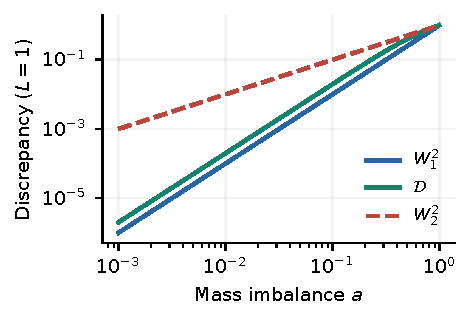
\includegraphics[width=.48\textwidth]{figures/transport_bounds.pdf}
\caption{Exact two-point example from Appendix~\ref{app:proofs}. The midpoint discrepancy controls $W_1^2$ but need not control $W_2^2$ by a universal linear constant. Curves are analytic, not learned-model estimates.}\label{fig:bounds}\end{figure}
\subsection{Historical Additional-Geometry Pilots}
The following historical runs use the legacy metric estimator and one training seed. Its kernel was fitted from generated and target points, and test metrics were monitored during development. We report final steps only, but historical tuning exposure remains. Values are exploratory and must not be pooled with the new fixed-kernel, three-seed tables. Paired-source tasks were adapted to target-only generation by retaining $x_1$; therefore the maze and hyperbolic rows do not reproduce the original source-to-target transport experiment.
Table~\ref{tab:legacy-extra} records all matching historical final-step runs, including repeated configurations rather than selecting the best observed result.
\begin{table}[t]\caption{Historical additional-geometry pilots with their original estimator. Repeated task/method rows are separate configurations; these values are not comparable to the new fixed-kernel table.}\label{tab:legacy-extra}\centering\small\begin{tabular}{@{}llrrrr@{}}\toprule
Task & Method & Dimension & Steps & Legacy MMD$^2$ & Legacy sym. NN \\
\midrule
hyperbolic & Light RFM & 2 & 2000 & 0.0151 & 0.0269 \\
hyperbolic & R-MGM & 2 & 2000 & 0.0108 & 0.0089 \\
maze3v2 & Light RFM & 3 & 500 & 0.1210 & 0.1473 \\
maze3v2 & R-MGM & 3 & 500 & 0.2446 & 0.1293 \\
maze3v2 & R-MGM & 3 & 500 & 0.0009 & 0.0052 \\
maze4v2 & Light RFM & 3 & 500 & 0.0613 & 0.1321 \\
maze4v2 & R-MGM & 3 & 500 & 0.0050 & 0.0078 \\
simple\_bunny & Light RFM & 3 & 500 & 0.5121 & 0.3097 \\
simple\_bunny & R-MGM & 3 & 500 & 0.0023 & 0.0051 \\
wrapped\_spd & Light RFM & 3 & 2000 & 0.0051 & 0.1122 \\
wrapped\_spd & R-MGM & 3 & 2000 & 0.0096 & 0.1144 \\
wrapped\_torus & Light RFM & 5 & 2000 & 0.1912 & 0.5299 \\
wrapped\_torus & R-MGM & 5 & 2000 & 0.0007 & 0.1218 \\
wrapped\_spd & Light RFM & 6 & 1000 & 0.0101 & 0.3962 \\
wrapped\_spd & Light RFM & 10 & 1000 & 0.0067 & 0.7417 \\
wrapped\_spd & R-MGM & 6 & 1000 & 0.0296 & 0.4868 \\
wrapped\_spd & R-MGM & 6 & 1000 & 0.0087 & 0.4137 \\
wrapped\_spd & R-MGM & 10 & 1000 & 0.0169 & 0.8048 \\
wrapped\_torus & Light RFM & 10 & 1000 & 0.4044 & 1.6642 \\
wrapped\_torus & Light RFM & 20 & 1000 & 0.4979 & 3.6284 \\
wrapped\_torus & R-MGM & 10 & 1000 & 0.0010 & 0.3639 \\
wrapped\_torus & R-MGM & 20 & 1000 & 0.0010 & 0.7266 \\
\bottomrule\end{tabular}\end{table}
Wrapped-SPD vector dimensions 3, 6, 10 correspond to matrix sizes 2, 3, 4. They are synthetic data, not EEG covariance models. The high-dimensional torus pilots cover dimensions 5, 10 and 20 only; they are not the full author scaling sweep.
Figure~\ref{fig:extra-volcano} shows the fixed-seed comparison for Volcano.
\begin{figure*}[t]\centering
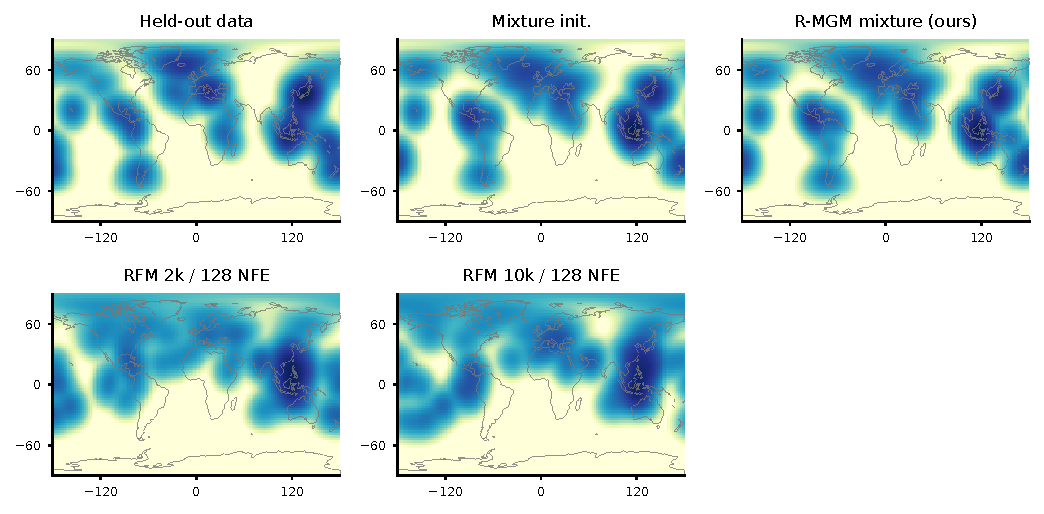
\includegraphics[width=\textwidth]{figures/volcano_comparison.pdf}
\caption{Volcano: fixed test target and training seed 0. Columns are labeled with their generator or flow training budget. Common-bandwidth sample KDEs use the same scale within this figure; these are not likelihood plots.}\label{fig:extra-volcano}\end{figure*}
Figure~\ref{fig:extra-earthquake} shows the fixed-seed comparison for Earthquake.
\begin{figure*}[t]\centering
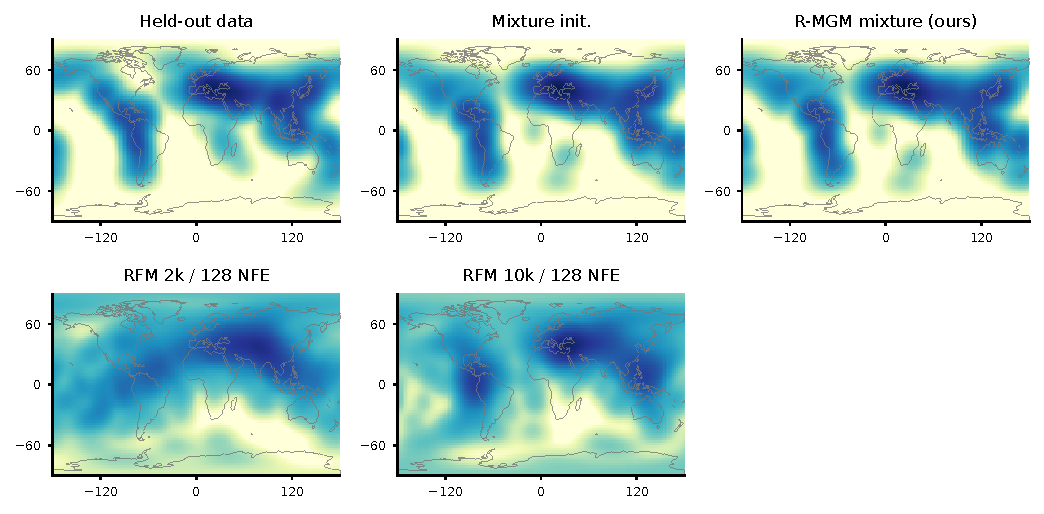
\includegraphics[width=\textwidth]{figures/earthquake_comparison.pdf}
\caption{Earthquake: fixed test target and training seed 0. Columns are labeled with their generator or flow training budget. Common-bandwidth sample KDEs use the same scale within this figure; these are not likelihood plots.}\label{fig:extra-earthquake}\end{figure*}
Figure~\ref{fig:extra-flood} shows the fixed-seed comparison for Flood.
\begin{figure*}[t]\centering
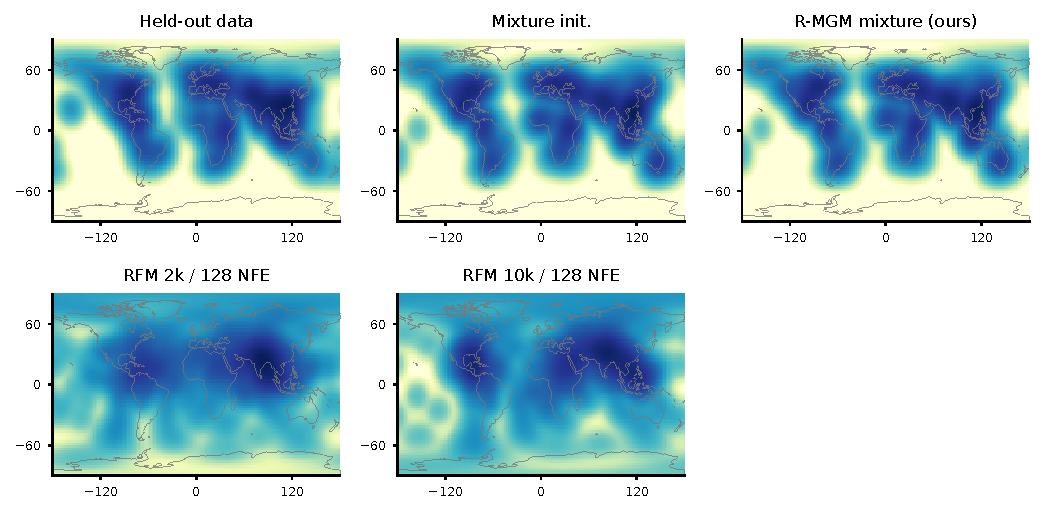
\includegraphics[width=\textwidth]{figures/flood_comparison.pdf}
\caption{Flood: fixed test target and training seed 0. Columns are labeled with their generator or flow training budget. Common-bandwidth sample KDEs use the same scale within this figure; these are not likelihood plots.}\label{fig:extra-flood}\end{figure*}
Figure~\ref{fig:extra-fire} shows the fixed-seed comparison for Fire.
\begin{figure*}[t]\centering
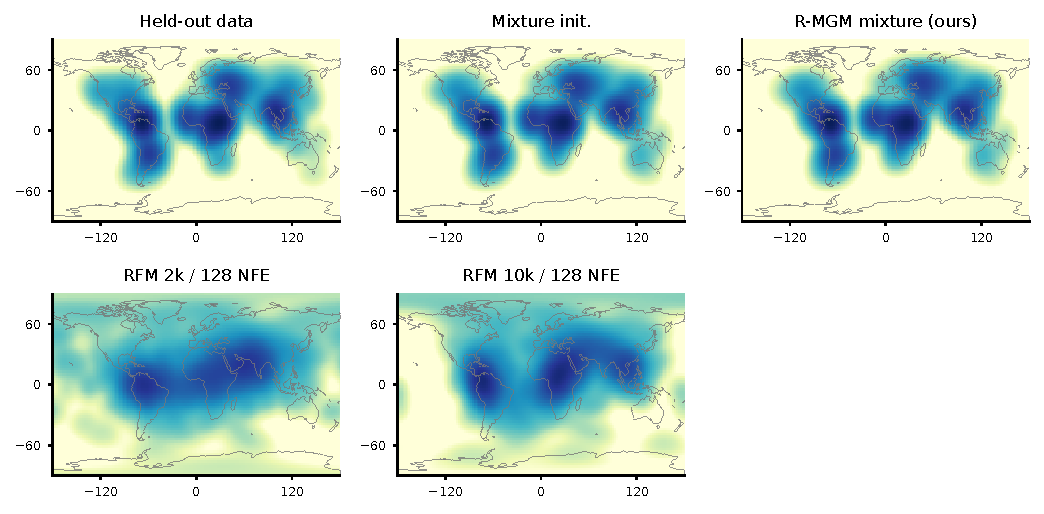
\includegraphics[width=\textwidth]{figures/fire_comparison.pdf}
\caption{Fire: fixed test target and training seed 0. Columns are labeled with their generator or flow training budget. Common-bandwidth sample KDEs use the same scale within this figure; these are not likelihood plots.}\label{fig:extra-fire}\end{figure*}
Figure~\ref{fig:extra-general} shows the fixed-seed comparison for General.
\begin{figure*}[t]\centering
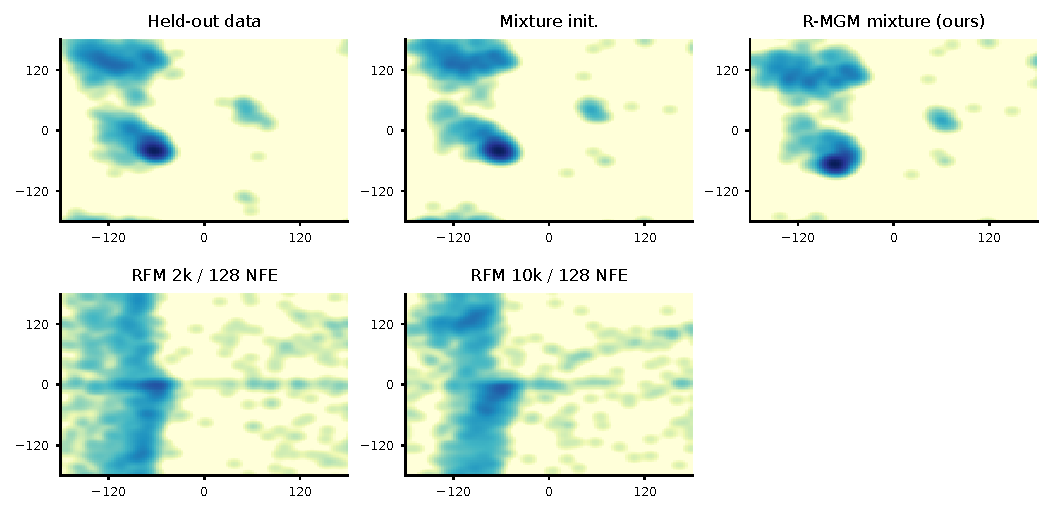
\includegraphics[width=\textwidth]{figures/general_comparison.pdf}
\caption{General: fixed test target and training seed 0. Columns are labeled with their generator or flow training budget. Common-bandwidth sample KDEs use the same scale within this figure; these are not likelihood plots.}\label{fig:extra-general}\end{figure*}
Figure~\ref{fig:extra-glycine} shows the fixed-seed comparison for Glycine.
\begin{figure*}[t]\centering
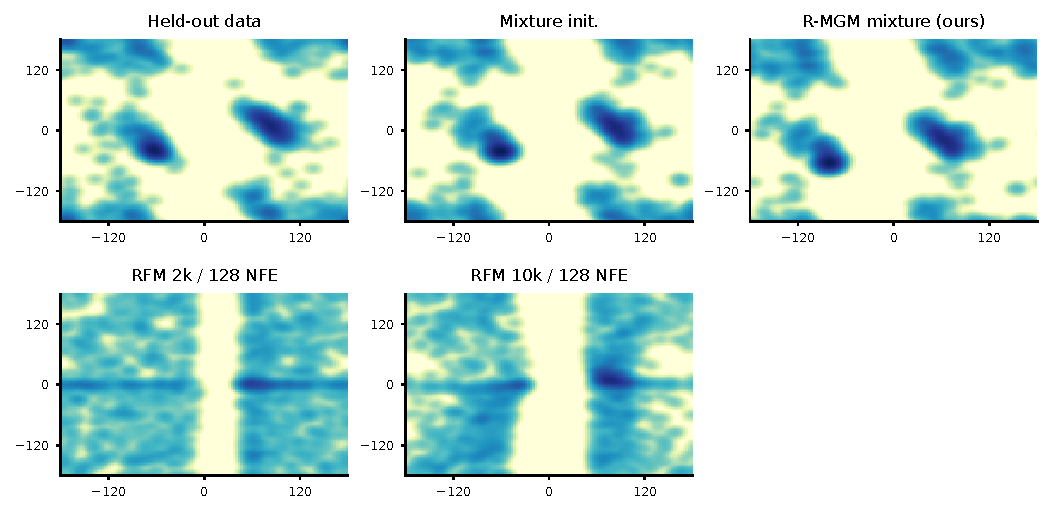
\includegraphics[width=\textwidth]{figures/glycine_comparison.pdf}
\caption{Glycine: fixed test target and training seed 0. Columns are labeled with their generator or flow training budget. Common-bandwidth sample KDEs use the same scale within this figure; these are not likelihood plots.}\label{fig:extra-glycine}\end{figure*}
Figure~\ref{fig:extra-proline} shows the fixed-seed comparison for Proline.
\begin{figure*}[t]\centering
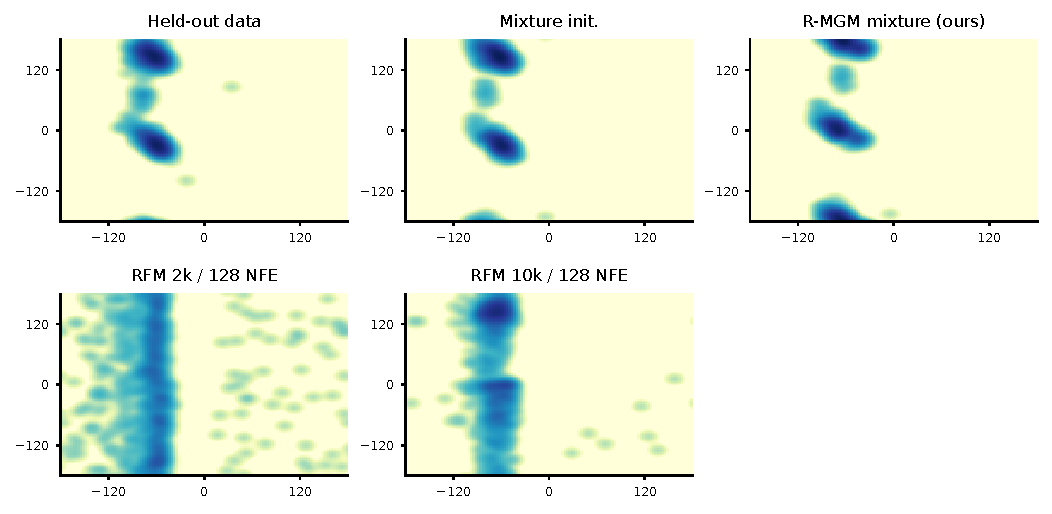
\includegraphics[width=\textwidth]{figures/proline_comparison.pdf}
\caption{Proline: fixed test target and training seed 0. Columns are labeled with their generator or flow training budget. Common-bandwidth sample KDEs use the same scale within this figure; these are not likelihood plots.}\label{fig:extra-proline}\end{figure*}
Figure~\ref{fig:extra-prepro} shows the fixed-seed comparison for Pre-Pro.
\begin{figure*}[t]\centering
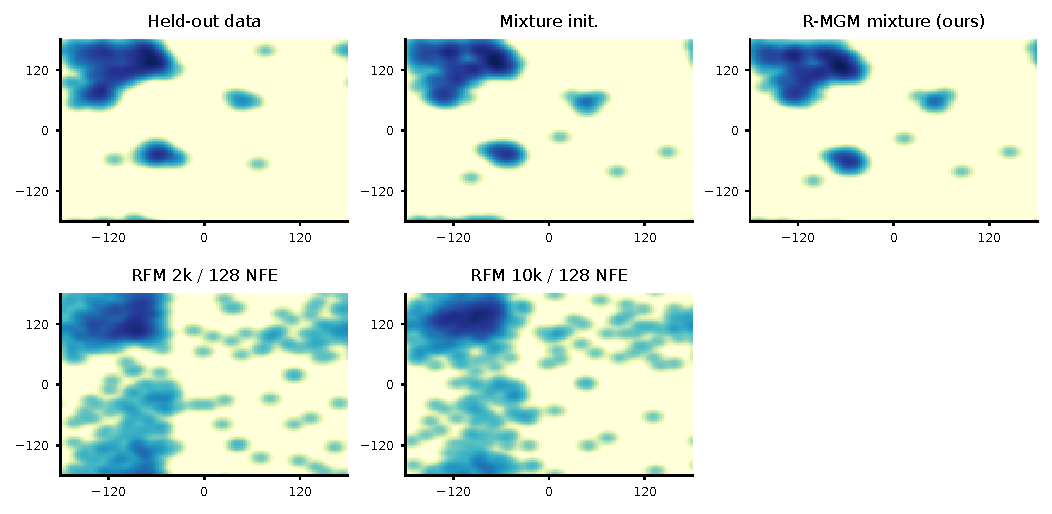
\includegraphics[width=\textwidth]{figures/prepro_comparison.pdf}
\caption{Pre-Pro: fixed test target and training seed 0. Columns are labeled with their generator or flow training budget. Common-bandwidth sample KDEs use the same scale within this figure; these are not likelihood plots.}\label{fig:extra-prepro}\end{figure*}
Figure~\ref{fig:extra-rna} shows the fixed-seed comparison for RNA (7D).
\begin{figure*}[t]\centering
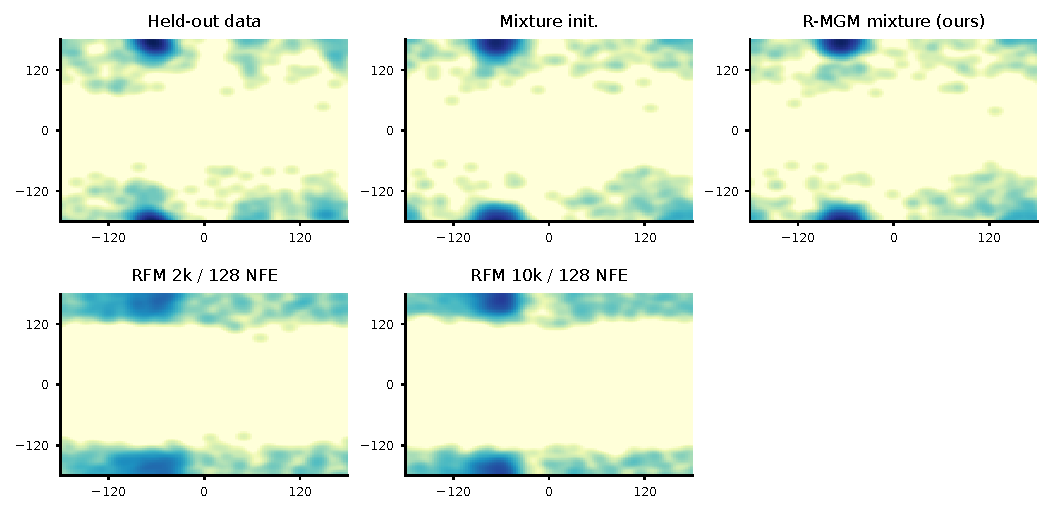
\includegraphics[width=\textwidth]{figures/rna_comparison.pdf}
\caption{RNA (7D): fixed test target and training seed 0. Columns are labeled with their generator or flow training budget. Common-bandwidth sample KDEs use the same scale within this figure; these are not likelihood plots.}\label{fig:extra-rna}\end{figure*}
\subsection{Final-Checkpoint Exploratory Mesh Results}
Each row is a single seed-0 model trained for 800 iterations. Values average three generated draws against the same 1,024 held-out targets. The plus/minus below is Monte Carlo sample SD, not training-seed variation. All kernels and coverage radii use a fixed training reference. The targets retain historical test exposure; final-checkpoint reevaluation does not erase it.
Table~\ref{tab:mesh} gives the final-checkpoint surface results.
\begin{table}[t]\caption{Exploratory mesh models: means and Monte Carlo SD over three draws from a single trained model per row. These are ambient sample metrics, not intrinsic likelihoods.}\label{tab:mesh}\centering\small\begin{tabular}{@{}llrrrr@{}}\toprule
Target & Generator & MMD$^2\times10^3$ & Ambient sym. NN & Coverage & Mean feasibility \\
\midrule
bunny10 & Projected mixture & $1.019\pm0.298$ & $0.043\pm0.000$ & $0.384\pm0.017$ & $2.8e-09$ \\
bunny10 & Soft sphere map & $33.905\pm0.992$ & $0.085\pm0.000$ & $0.248\pm0.012$ & $2.9e-09$ \\
bunny10 & Sphere-map mixture & $1.321\pm0.570$ & $0.042\pm0.000$ & $0.383\pm0.005$ & $3.1e-09$ \\
bunny100 & Projected mixture & $1.586\pm0.503$ & $0.063\pm0.001$ & $0.321\pm0.007$ & $3.2e-09$ \\
bunny100 & Soft sphere map & $75.212\pm7.842$ & $0.084\pm0.002$ & $0.161\pm0.007$ & $3.7e-09$ \\
bunny100 & Sphere-map mixture & $2.381\pm0.576$ & $0.056\pm0.001$ & $0.317\pm0.020$ & $3.1e-09$ \\
bunny50 & Projected mixture & $0.524\pm0.208$ & $0.043\pm0.001$ & $0.429\pm0.017$ & $2.7e-09$ \\
bunny50 & Soft sphere map & $53.416\pm2.984$ & $0.111\pm0.002$ & $0.158\pm0.014$ & $3.2e-09$ \\
bunny50 & Sphere-map mixture & $1.156\pm0.096$ & $0.048\pm0.001$ & $0.375\pm0.005$ & $2.9e-09$ \\
spot10 & Projected mixture & $0.751\pm0.398$ & $0.027\pm0.001$ & $0.453\pm0.035$ & $1.8e-09$ \\
spot10 & Soft sphere map & $47.778\pm1.717$ & $0.093\pm0.001$ & $0.189\pm0.004$ & $2.4e-09$ \\
spot10 & Sphere-map mixture & $1.167\pm0.601$ & $0.028\pm0.001$ & $0.444\pm0.013$ & $2.1e-09$ \\
spot100 & Projected mixture & $1.212\pm0.210$ & $0.052\pm0.002$ & $0.308\pm0.029$ & $2.8e-09$ \\
spot100 & Soft sphere map & $17.464\pm2.354$ & $0.061\pm0.002$ & $0.168\pm0.021$ & $2.8e-09$ \\
spot100 & Sphere-map mixture & $1.027\pm0.152$ & $0.047\pm0.001$ & $0.268\pm0.009$ & $2.8e-09$ \\
spot50 & Projected mixture & $1.897\pm0.666$ & $0.042\pm0.000$ & $0.388\pm0.008$ & $3.0e-09$ \\
spot50 & Soft sphere map & $35.720\pm3.309$ & $0.082\pm0.001$ & $0.153\pm0.010$ & $2.7e-09$ \\
spot50 & Sphere-map mixture & $2.516\pm0.586$ & $0.041\pm0.000$ & $0.385\pm0.005$ & $2.7e-09$ \\
\bottomrule\end{tabular}\end{table}
Surface feasibility measures mean distance to a second closest-point projection. It is not an intrinsic density metric or a certificate of bijective parameterization. The soft map interpolates radii from mesh-vertex directions and then projects; it is not the separate ray-intersection utility.
Figure~\ref{fig:surface-bunny10} gives the full parameterization comparison for bunny10.
\begin{figure*}[t]\centering
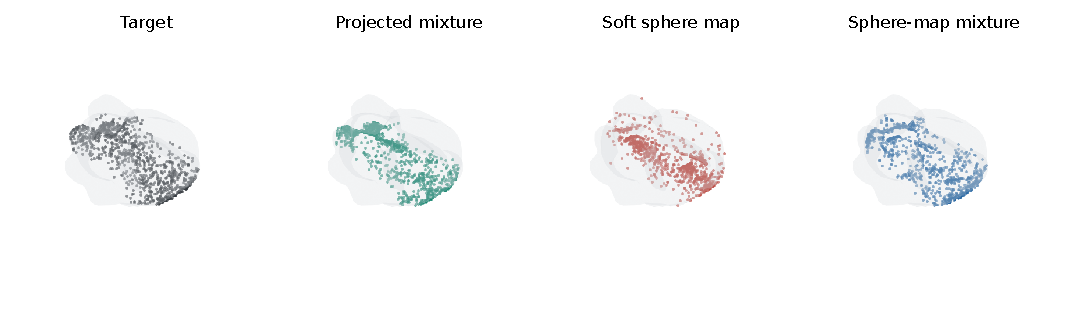
\includegraphics[width=\textwidth]{figures/bunny10_surface.pdf}
\caption{bunny10: one fixed seed-0 final checkpoint per variant, common cameras and 1,024 points. The loss is a local projection surrogate, not the spectral-path construction.}\label{fig:surface-bunny10}\end{figure*}
Figure~\ref{fig:surface-bunny50} gives the full parameterization comparison for bunny50.
\begin{figure*}[t]\centering
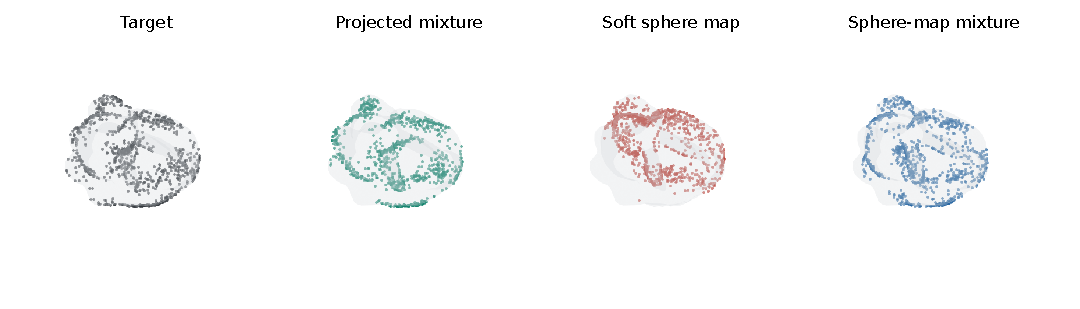
\includegraphics[width=\textwidth]{figures/bunny50_surface.pdf}
\caption{bunny50: one fixed seed-0 final checkpoint per variant, common cameras and 1,024 points. The loss is a local projection surrogate, not the spectral-path construction.}\label{fig:surface-bunny50}\end{figure*}
Figure~\ref{fig:surface-bunny100} gives the full parameterization comparison for bunny100.
\begin{figure*}[t]\centering
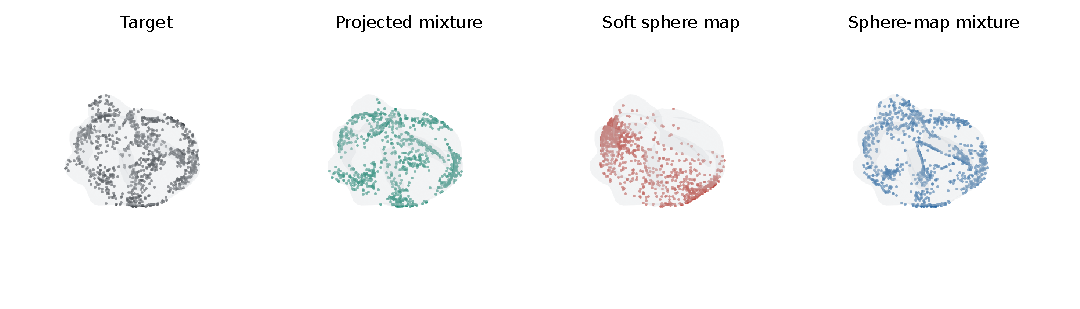
\includegraphics[width=\textwidth]{figures/bunny100_surface.pdf}
\caption{bunny100: one fixed seed-0 final checkpoint per variant, common cameras and 1,024 points. The loss is a local projection surrogate, not the spectral-path construction.}\label{fig:surface-bunny100}\end{figure*}
Figure~\ref{fig:surface-spot10} gives the full parameterization comparison for spot10.
\begin{figure*}[t]\centering
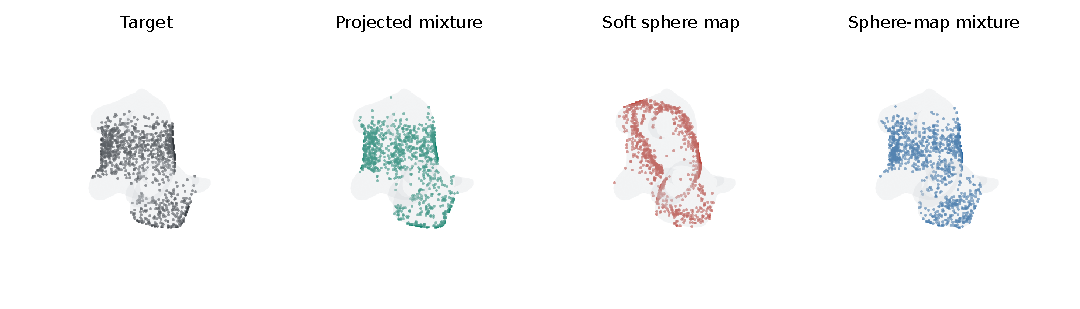
\includegraphics[width=\textwidth]{figures/spot10_surface.pdf}
\caption{spot10: one fixed seed-0 final checkpoint per variant, common cameras and 1,024 points. The loss is a local projection surrogate, not the spectral-path construction.}\label{fig:surface-spot10}\end{figure*}
Figure~\ref{fig:surface-spot50} gives the full parameterization comparison for spot50.
\begin{figure*}[t]\centering
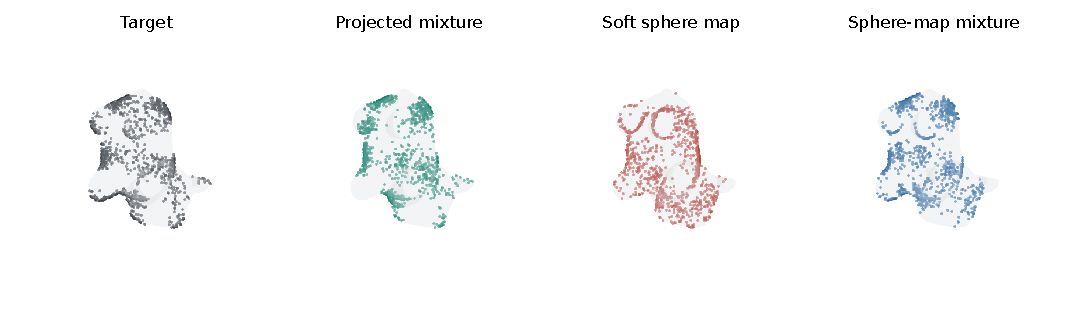
\includegraphics[width=\textwidth]{figures/spot50_surface.pdf}
\caption{spot50: one fixed seed-0 final checkpoint per variant, common cameras and 1,024 points. The loss is a local projection surrogate, not the spectral-path construction.}\label{fig:surface-spot50}\end{figure*}
Figure~\ref{fig:surface-spot100} gives the full parameterization comparison for spot100.
\begin{figure*}[t]\centering
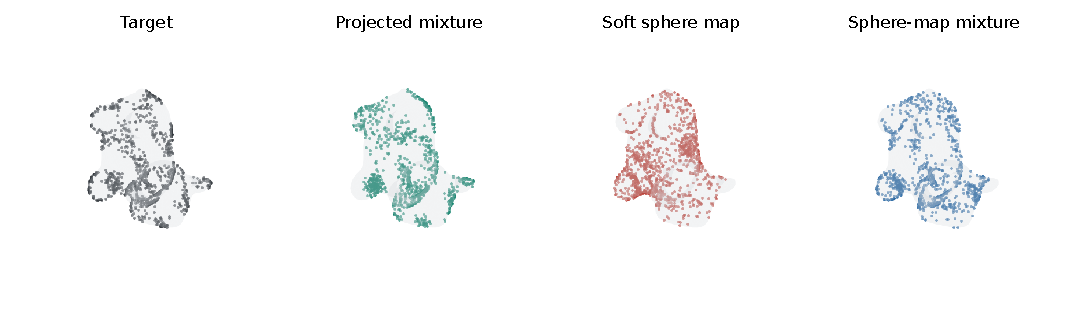
\includegraphics[width=\textwidth]{figures/spot100_surface.pdf}
\caption{spot100: one fixed seed-0 final checkpoint per variant, common cameras and 1,024 points. The loss is a local projection surrogate, not the spectral-path construction.}\label{fig:surface-spot100}\end{figure*}
